\subsection{\mlblinkui} \label{subsect:case-study:impl:ml-blink-ui}

As described in section \ref{sect:case-study:intro}, the \mlblinkui allows users to match images of distinct datasets of the same location in the night sky. The goal is to provide intuitive feedback about the quality of the current matching to the user, where a good matching receives a better score than a bad one. \newline

The different steps taken to process a matching can be summarized as follows: computing the region of interest (ROI), smoothing, binarization, object detection, object size normalization, and computing accuracy. These steps in conjunction define the algorithm used to compute the quality of a matching, and it is referred to as the matching algorithm. \newline

The matching algorithm runs in the main thread (also known as the UI thread) in the client hardware that renders the \mlblinkui; which might be a fast desktop, or a slow mobile device. Therefore, it is important that the matching algorithm runs fast so that the UI thread does not ``freeze'' and the user experience degrade. \newline

Every time the user changes the position of the \panstarrs image, a ``debounced'' function is created. A debounced function allows to wait a specified number of milliseconds before invoking another function. This allows the \mlblinkui to avoid computing the aforementioned algorithm every time the user changes the position of the \panstarrs image, and instead wait until 250 \si{\milli\second} have elapsed -- and no further position or transformation has occurred -- to execute the matching algorithm. \newline

In order to better illustrate how the matching algorithm works, the following subsections will use figure \ref{fig:mission-0} as an example. It is worth nothing that while all of these steps are performed when determining the accuracy of a matching, only step \ref{subsubsect:case-study:impl:roi} is actually drawn behind the scenes in the UI. The arrays which represent the rest of these steps are only stored in memory, since there is no need to draw them on the UI. Additionally, except for the accuracy computation, all of these steps are only performed once for the \usno image when it is loaded, since it is static and there is no need to re--compute the same thing again.

\begin{figure}[H]
    \centering
    \begin{subfigure}{.5\textwidth}
      \centering
      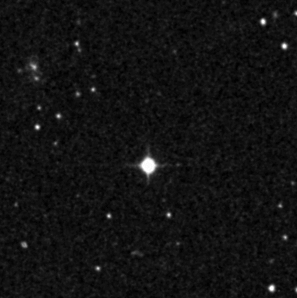
\includegraphics[
            width=\textwidth,
            height=0.30\textheight,
            keepaspectratio
        ]{report/images/image-matching/usno-0-blue1.png}
      \caption{\usno}
      \label{fig:a:usno-0-blue1}
    \end{subfigure}%
    \begin{subfigure}{.5\textwidth}
      \centering
      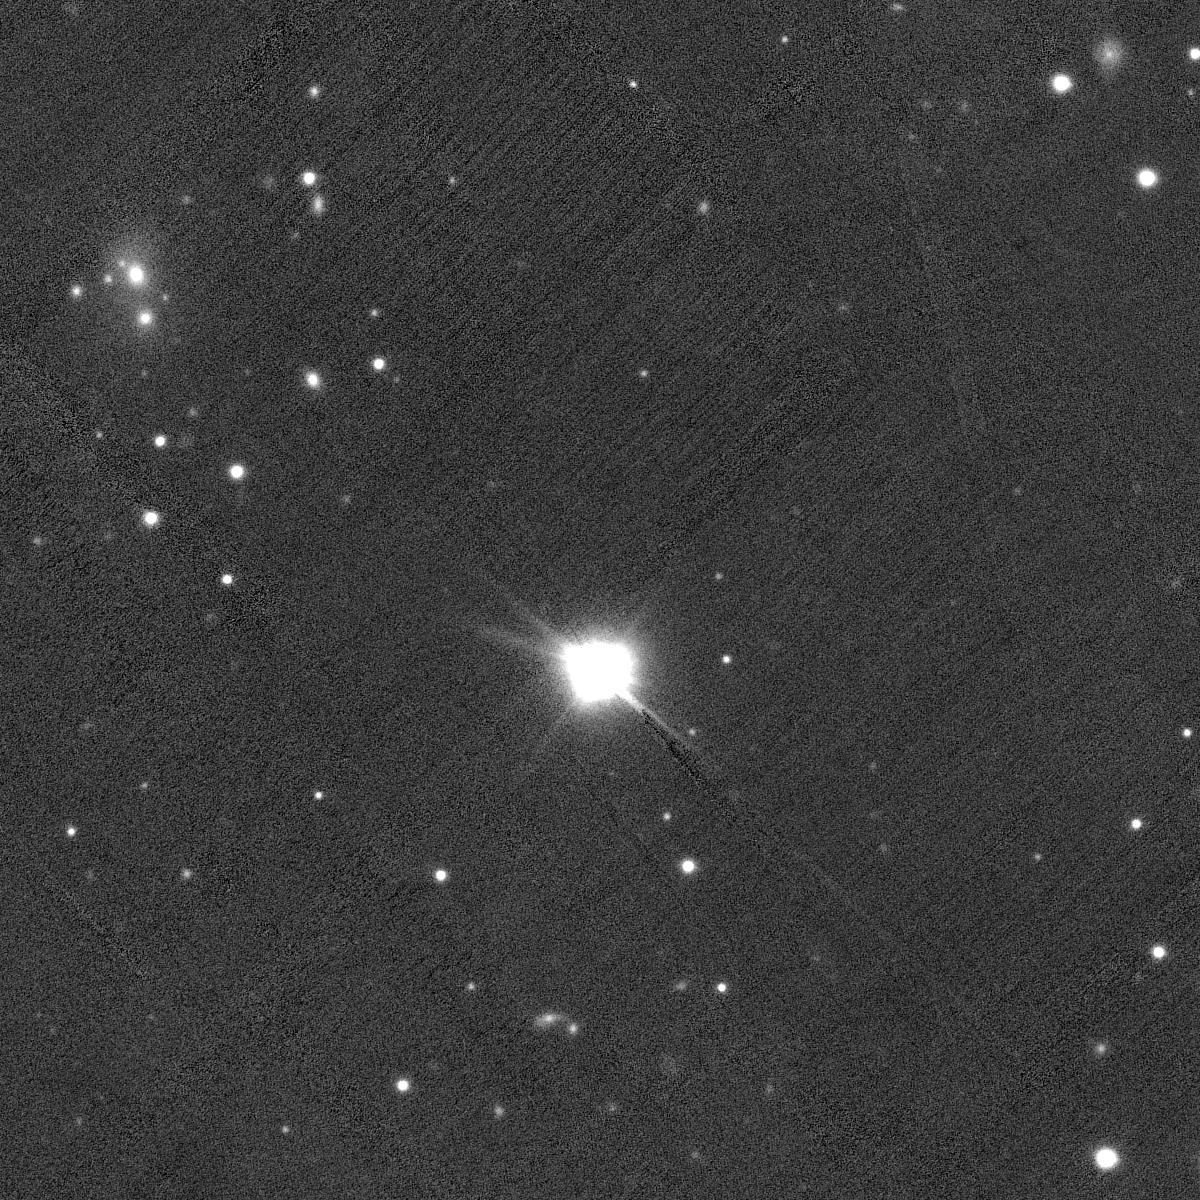
\includegraphics[
            width=\textwidth,
            height=0.30\textheight,
            keepaspectratio
      ]{report/images/image-matching/panstarr-0-g.png}
      \caption{\panstarrs}
      \label{fig:b:panstarr-0-g}
    \end{subfigure}
    \caption{Figures \ref{fig:a:usno-0-blue1} and \ref{fig:b:panstarr-0-g} show pictures taken from the same location in the night sky from \usno and \panstarrs respectively.}
    \label{fig:mission-0}
\end{figure}

As the user moves or transforms the \panstarrs image in the UI, the following debounced steps are executed:

\subsubsection{ROI} \label{subsubsect:case-study:impl:roi}

The ROI is defined as a square of 200 pixels placed on top of the center of the \usno image. The resulting ROI of the \usno image is shown in figure \ref{fig:a:usno-0-blue1-roi}. The ROI of the \panstarrs image is defined from the exact location, which means that in order to match the two images, the user must place the \panstarrs on top of the \usno image, otherwise the resulting ROI will be completely dark (i.e. no pixels from the \panstarrs image were found in the same location as the \usno ROI). Figure \ref{fig:b:panstarr-0-g-roi} shows the resulting ROI of the \panstarrs image as if it was positioned exactly on top of the \usno image in the UI. \newline

The choice to use a ROI to measure the quality of a matching was made based on the requirements established for the construction of the datasets used in the case--study (see section \ref{sect:meth:datasets}), as well as an approach to aid the design of an algorithm that evaluated faster.

\begin{figure}[H]
    \centering
    \begin{subfigure}{.5\textwidth}
      \centering
      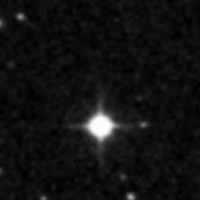
\includegraphics[
            width=0.75\textwidth,
            height=\textheight,
            keepaspectratio
        ]{report/images/image-matching/usno-0-blue1-roi.png}
      \caption{\usno ROI}
      \label{fig:a:usno-0-blue1-roi}
    \end{subfigure}%
    \begin{subfigure}{.5\textwidth}
      \centering
      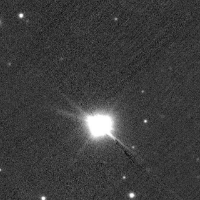
\includegraphics[
            width=0.75\textwidth,
            height=\textheight,
            keepaspectratio
      ]{report/images/image-matching/panstarr-0-g-roi.png}
      \caption{\panstarrs ROI}
      \label{fig:b:panstarr-0-g-roi}
    \end{subfigure}
    \caption{Resulting ROI from the figures shown in figure \ref{fig:mission-0}. The ROI were computed as if the \panstarrs image was placed exactly on top of the \usno image in the UI .}
    \label{fig:mission-0:roi}
\end{figure}

\subsubsection{Smoothing} \label{subsubsect:case-study:impl:smooth}
Once the ROI has been computed for both images, the pixel value intensities of the RGBA channels of each image in their respective ROI are retrieved. Since the images are in gray--scale format, all RGB pixel value intensities at the same location are equal, which means that the remaining computations can be performed using a single channel. As a result, only the pixel value intensities of the R channel are smoothed using a mean filter, which facilitates object detection in the upcoming steps. \newline

The mean filter uses a $3 \times 3$ kernel which scans the entire ROI of each image and replaces the center pixel where the kernel is located at with the mean pixel value intensity of the entire ROI of each image. The mean pixel value intensity is also used for out--of--boundary pixels when placing the kernel in the border pixels of the ROI.

\subsubsection{Binarization} \label{subsubsect:case-study:impl:binarization}
The next step is to binarize the smoothed pixel value intensities of each image's ROI. The binarization process simply replaces all pixel value intensities larger than a specified threshold with 255, while pixel value intensities less or equal to the threshold are set to 0. Figure \ref{fig:mission-0:bw} shows the resulting ROI after both images have been binarized. The matching algorithm uses a fixed threshold of 80 for \usno and 110 for \panstarrs.

\begin{figure}[H]
    \centering
    \begin{subfigure}{.5\textwidth}
      \centering
      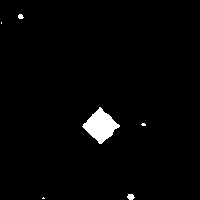
\includegraphics[
            width=0.75\textwidth,
            height=\textheight,
            keepaspectratio
        ]{report/images/image-matching/usno-0-blue1-bw.png}
      \caption{Binarized \usno}
      \label{fig:a:usno-0-blue1-bw}
    \end{subfigure}%
    \begin{subfigure}{.5\textwidth}
      \centering
      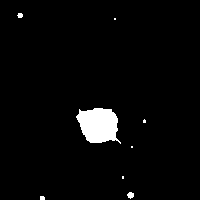
\includegraphics[
            width=0.75\textwidth,
            height=\textheight,
            keepaspectratio
      ]{report/images/image-matching/panstarr-0-g-bw.png}
      \caption{Binarized \panstarrs}
      \label{fig:b:panstarr-0-g-bw}
    \end{subfigure}
    \caption{Binarization result using a threshold value of 80 for figure \ref{fig:a:usno-0-blue1-bw} and 110 for figure \ref{fig:b:panstarr-0-g-bw}.}
    \label{fig:mission-0:bw}
\end{figure}

While a binarization technique that automatically finds what threshold to use could have been implemented, a fixed threshold is computationally faster and simpler. However, due to the threshold value not being optimal for all observations, it is also possible that a fixed threshold might mistakenly label a dark section as background, even if it is an object.

\subsubsection{Object Detection} \label{subsubsect:case-study:impl:objects}
The binarized ROI are then fed through an object detection algorithm. The object detection algorithm uses connected components to label all pixels connected to an object before proceeding with the next pixel. Since the input image is binarized, any object to be identified must have a pixel value intensity of 255. \newline

The algorithm works by first filtering the entire array of pixels by those which are cataloged as an object. Once these have been found, a kernel of size $3 \times 3$ placed on top of such pixels is used to find its neighbors. The neighbors are then filtered by those that are objects and have not been labeled yet. Following that, each of these neighbors are labeled using the label of that connected component, and kept track of in a queue data structure for follow up labelling. Only once all these neighbors have been labeled (i.e. the queue is empty), the algorithm continues with the next pixel value intensity cataloged as an object. \newline

Figure \ref{fig:mission-0:objects} shows the connected components found by the object detection algorithm in each of the images' ROI.

\begin{figure}[H]
    \centering
    \begin{subfigure}{.5\textwidth}
      \centering
      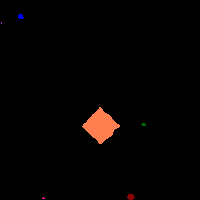
\includegraphics[
            width=0.75\textwidth,
            height=\textheight,
            keepaspectratio
        ]{report/images/image-matching/usno-0-blue1-objects.png}
      \caption{Objects in \usno}
      \label{fig:a:usno-0-blue1-objects}
    \end{subfigure}%
    \begin{subfigure}{.5\textwidth}
      \centering
      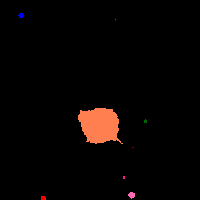
\includegraphics[
            width=0.75\textwidth,
            height=\textheight,
            keepaspectratio
      ]{report/images/image-matching/panstarr-0-g-objects.png}
      \caption{Objects in \panstarrs}
      \label{fig:b:panstarr-0-g-objects}
    \end{subfigure}
    \caption{Object detection result for both \usno (figure \ref{fig:a:usno-0-blue1-objects}) and \panstarrs (figure \ref{fig:b:panstarr-0-g-objects}) images' ROI. Note each of the objects label has been colorized for illustrative proposes only.}
    \label{fig:mission-0:objects}
\end{figure}

\subsubsection{Object Size Normalization} \label{subsubsect:case-study:impl:object-normalization}
The objects detected within each image's ROI are then normalized by replacing each of them by an equal sized square object. \usno objects are replaced by squares of size $9$, while objects of size $13$ for \panstarrs were found to result in a more intuitive score in the UI.  \newline

The object normalization algorithm takes the labeled objects as in figure \ref{fig:mission-0:objects}, and for each of them, computes its center of mass. The center of mass is calculated for the $x$--axis and $y$--axis in a similar way. The $x$--axis center of mass is computed by adding the row of each pixel defined within an object and dividing the resulting total by the number of pixels the object has. The same procedure is performed for the $y$--axis center of mass, but adding the column of each pixel defined within the object instead. Once the center of mass has been computed in both axis, a squared object of a specified size is placed on top of the object's center of mass. \newline

Figure \ref{fig:mission-0:equal-sized-objects} shows the resulting square objects after both the \usno and \panstarrs images' ROI objects size have been normalized.

\begin{figure}[H]
    \centering
    \begin{subfigure}{.5\textwidth}
      \centering
      
\includegraphics[
            width=0.75\textwidth,
            height=\textheight,
            keepaspectratio
        ]{report/images/image-matching/usno-0-blue1-equal-sized-objects.png}
      \caption{Equal sized objects in \usno}
      \label{fig:a:usno-0-blue1-equal-sized-objects}
    \end{subfigure}%
    \begin{subfigure}{.5\textwidth}
      \centering
      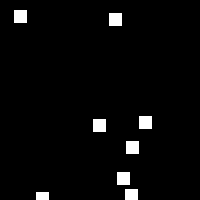
\includegraphics[
            width=0.75\textwidth,
            height=\textheight,
            keepaspectratio
      ]{report/images/image-matching/panstarr-0-g-equal-sized-objects.png}
      \caption{Equal sized objects in \panstarrs}
      \label{fig:b:panstarr-0-g-equal-sized-objects}
    \end{subfigure}
    \caption{Original objects from figure \ref{fig:mission-0:objects} replaced by equal sized objects in both \usno (figure \ref{fig:a:usno-0-blue1-equal-sized-objects}), and \panstarrs (figure \ref{fig:b:panstarr-0-g-equal-sized-objects}). Squared objects of size $9$ are used for \usno images and $13$ for \panstarrs images.}
    \label{fig:mission-0:equal-sized-objects}
\end{figure}

\subsubsection{Accuracy} \label{subsubsect:case-study:impl:accuracy}
The last step is to compute the accuracy of a matching. The accuracy of a matching is defined as the number of remaining bright pixel value intensities (pixel values equal to 255) when the \usno image is subtracted from the \panstarrs image. In other words, let the \usno image in figure \ref{fig:a:usno-0-blue1-equal-sized-objects} be $\text{xs}$, the \panstarrs image in figure \ref{fig:b:panstarr-0-g-equal-sized-objects} be $\text{ys}$, and $\text{zs}=\text{xs} - \text{ys}$. Then the accuracy is defined as: follows:

\begin{equation} \label{eq:accuracy}
    \text{accuracy} = 100 - \frac{|\text{zs} \in \{255\} | \times 100}{|\text{xs} \in \{255\} |}
\end{equation}

A fixed accuracy threshold of $80$\% is used in order to determine whether a mission is successfully completed or not. That is, if a user can create a matching where the accuracy as defined in equation \ref{eq:accuracy} is greater or equal to the $80$\% fixed threshold, then the mission is considered as successfully completed (unlikely to be an anomaly), while the opposite means it is possible there is an anomaly between the two images. \newline

It is worth noting the accuracy formula shown in equation \ref{eq:accuracy} only works in one--direction. That is, it exclusively works to identify objects in \usno that have disappeared (or significantly moved) in \panstarrs. An ideal solution would work both ways (i.e. it would also handle detecting appearing sources). Within the scope of this master thesis, the main goal was to create an evaluation technique for a matching that would make it difficult for an anomaly to be cataloged as a non--anomaly (since these are used by the \mlblink algorithm to learn what to recommend). The outlined solution was the best method implemented that could fairly well handle the different type of artifacts present in the two datasets, and avoid anomalies being cataloged as non--anomalies.
